\begin{frame}{Дублирование границ при декомпозиции}

\begin{figure}
\centering
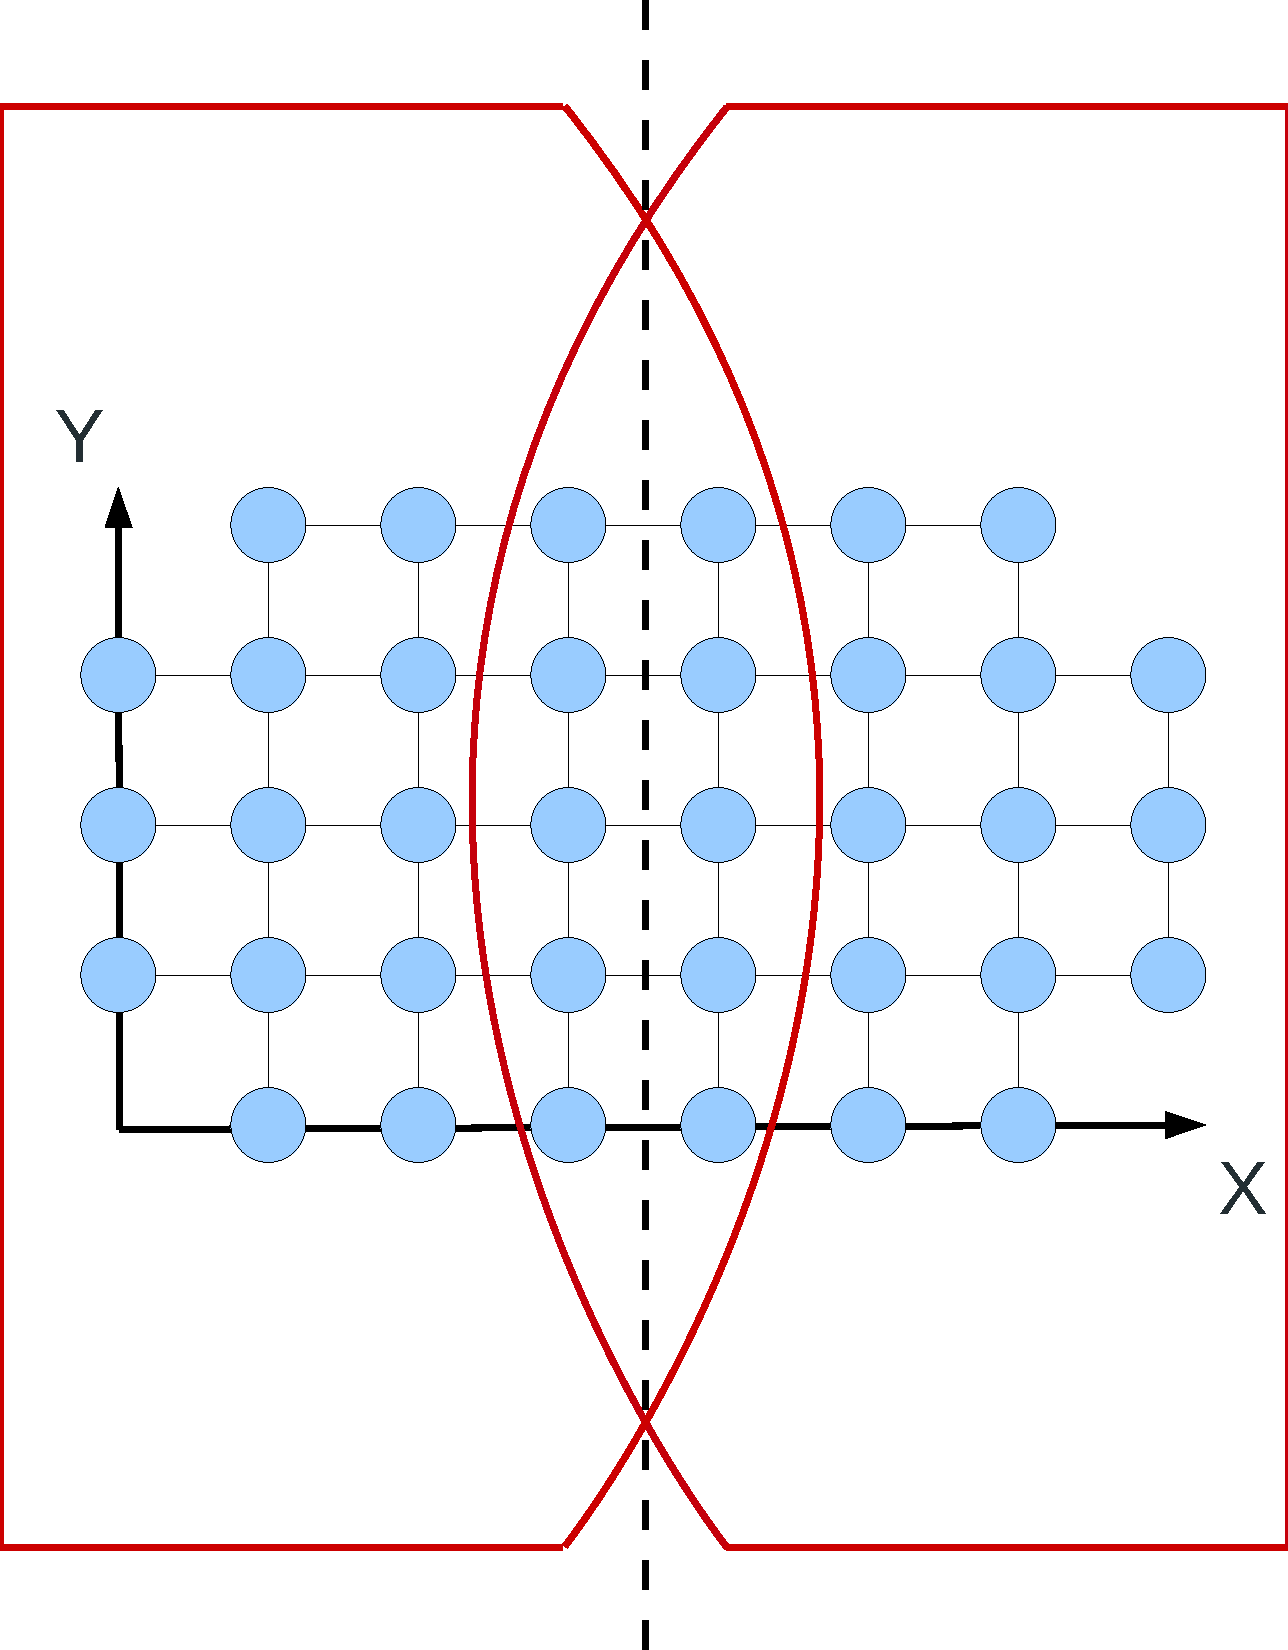
\includegraphics[height=2.5in]{artwork/pdf/decomp_0}
\end{figure}

\end{frame}

\begin{frame}{Данные в распределённой памяти}

\begin{figure}
\centering
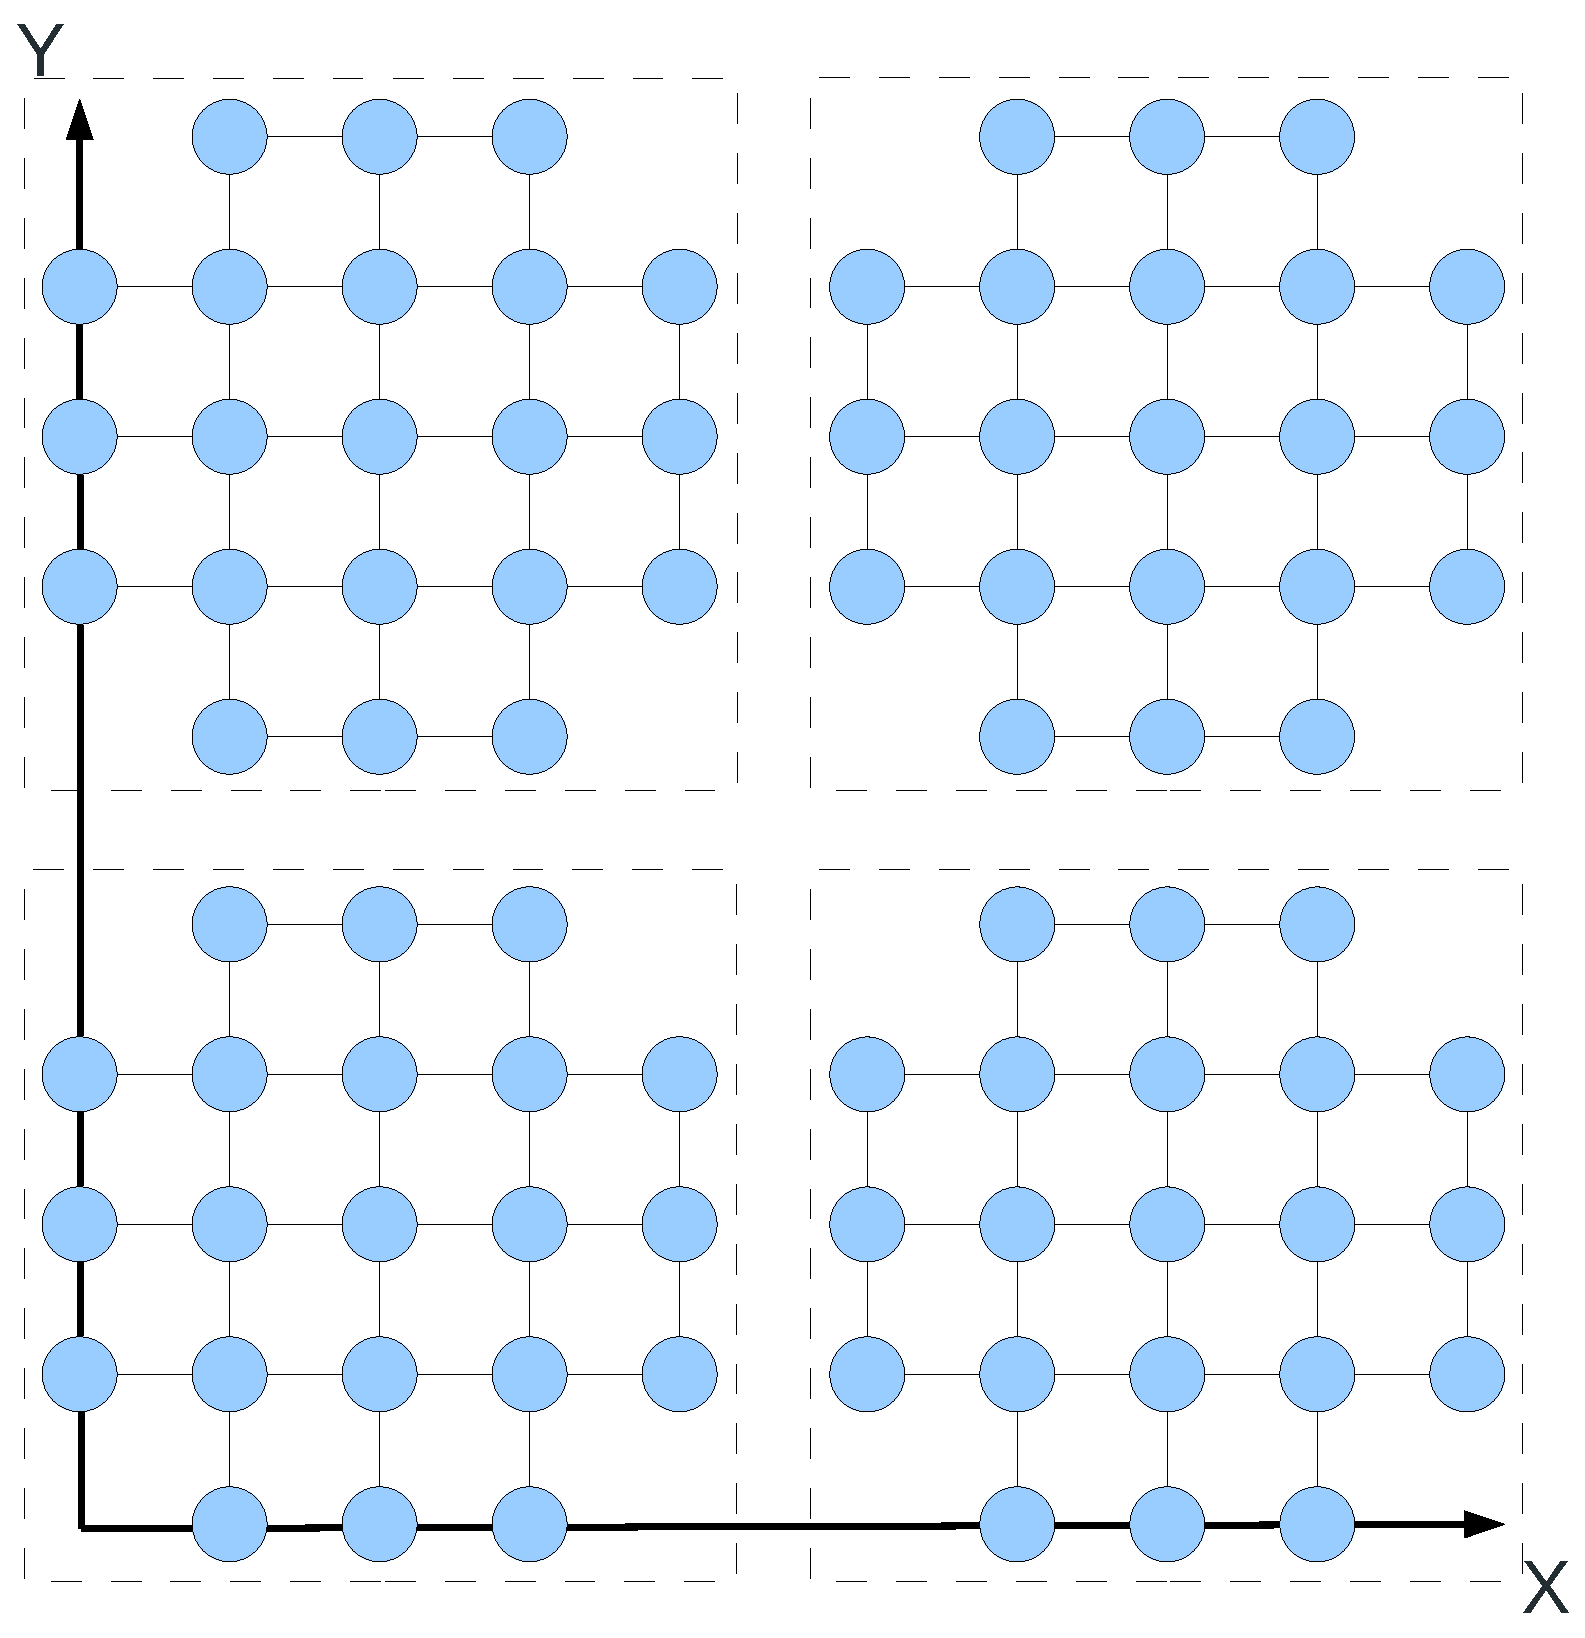
\includegraphics[height=2.5in]{artwork/pdf/decomp_1}
\end{figure}

\end{frame}

\begin{frame}{Параллельный расчёт внутренних узлов}

\begin{figure}
\centering
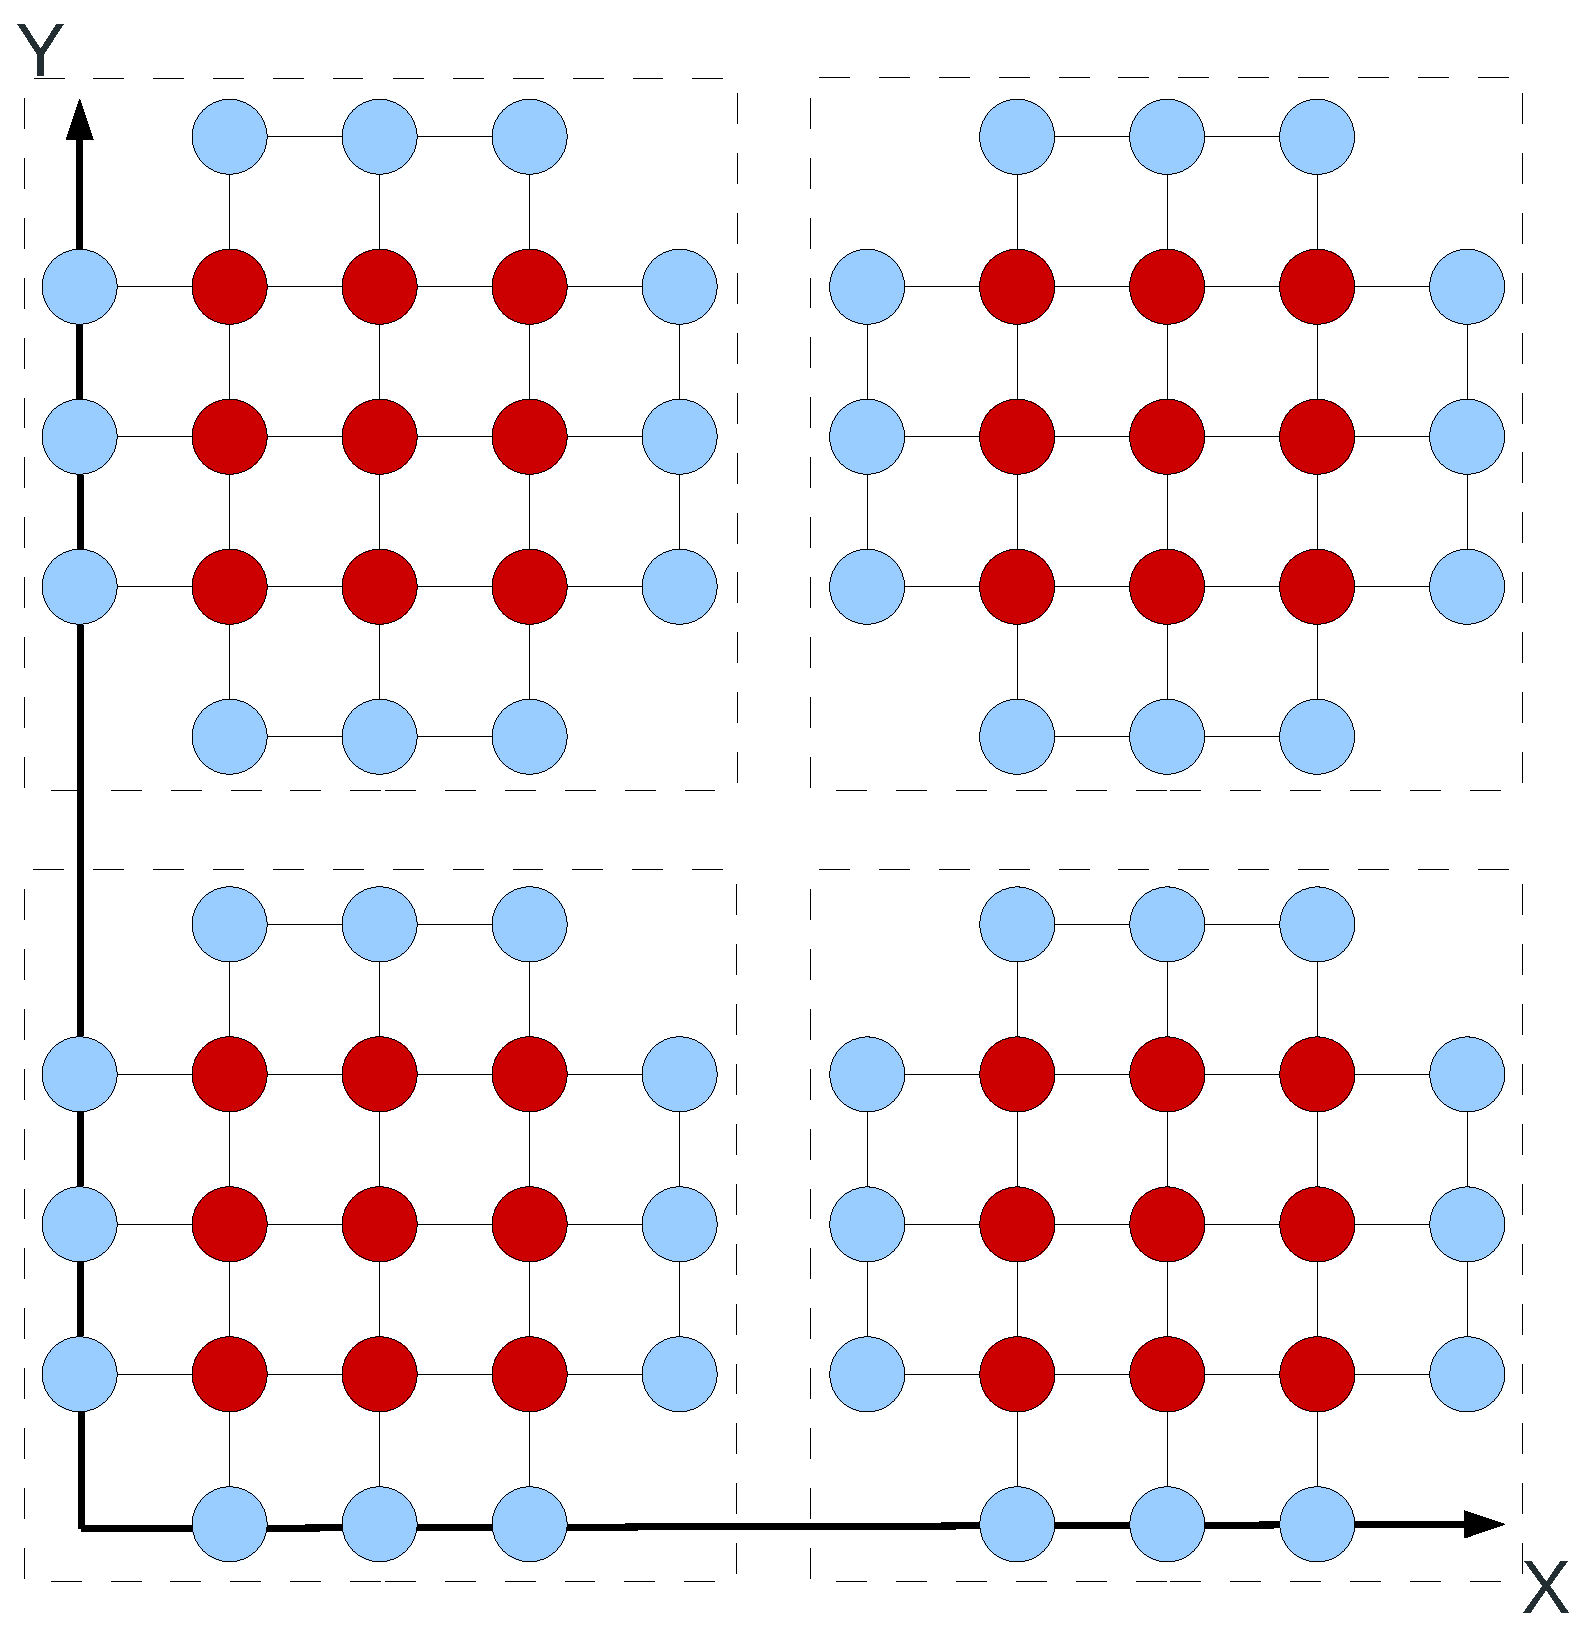
\includegraphics[height=2.5in]{artwork/pdf/decomp_2}
\end{figure}

\end{frame}


\begin{frame}{Синхронизация граничных узлов}

\begin{figure}
\centering
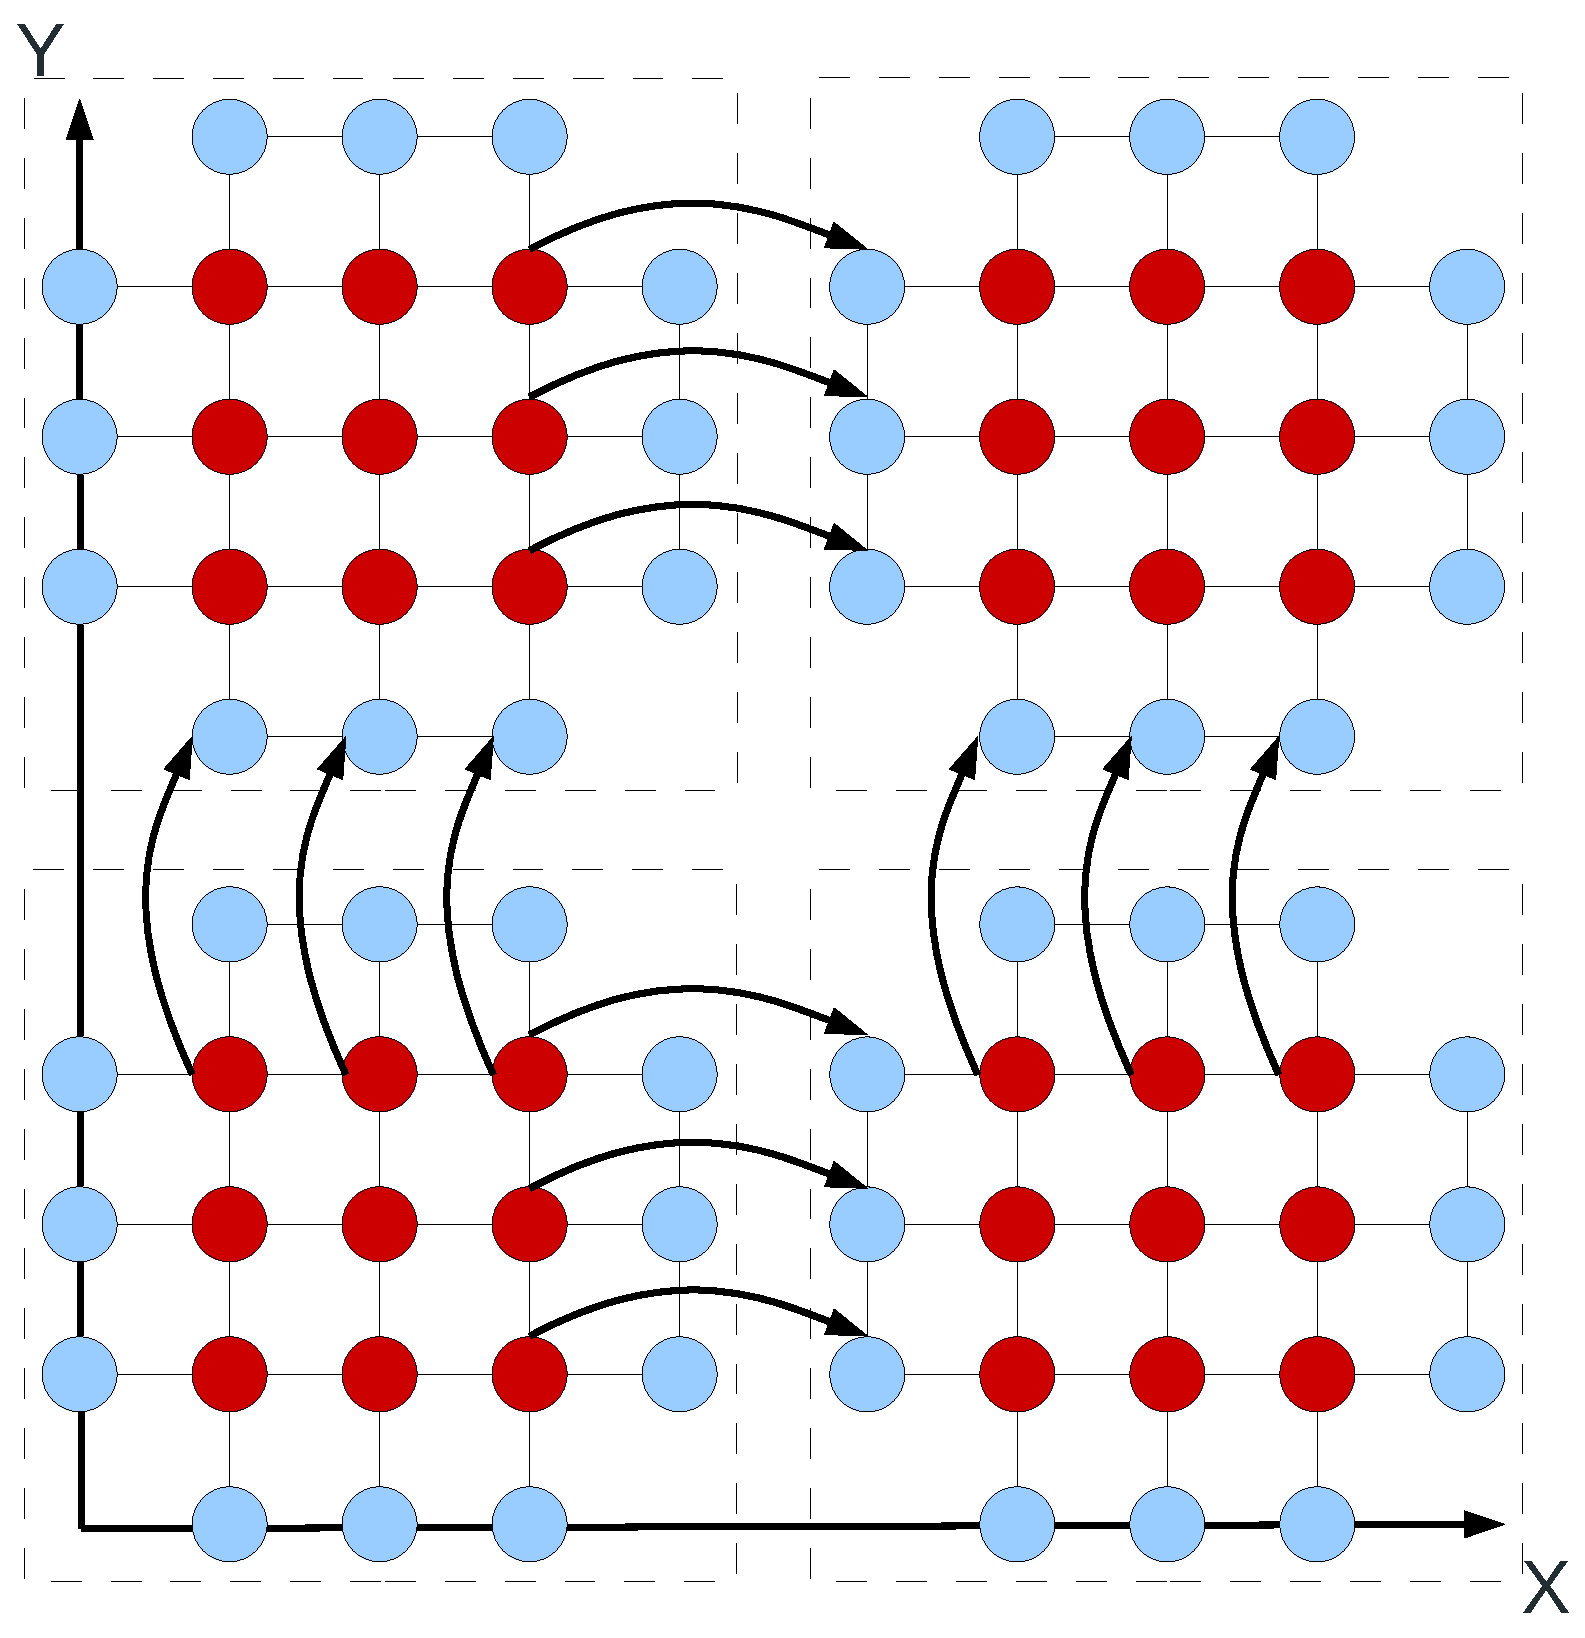
\includegraphics[height=2.5in]{artwork/pdf/decomp_3}
\end{figure}

\end{frame}


\begin{frame}{Синхронизация граничных узлов}

\begin{figure}
\centering
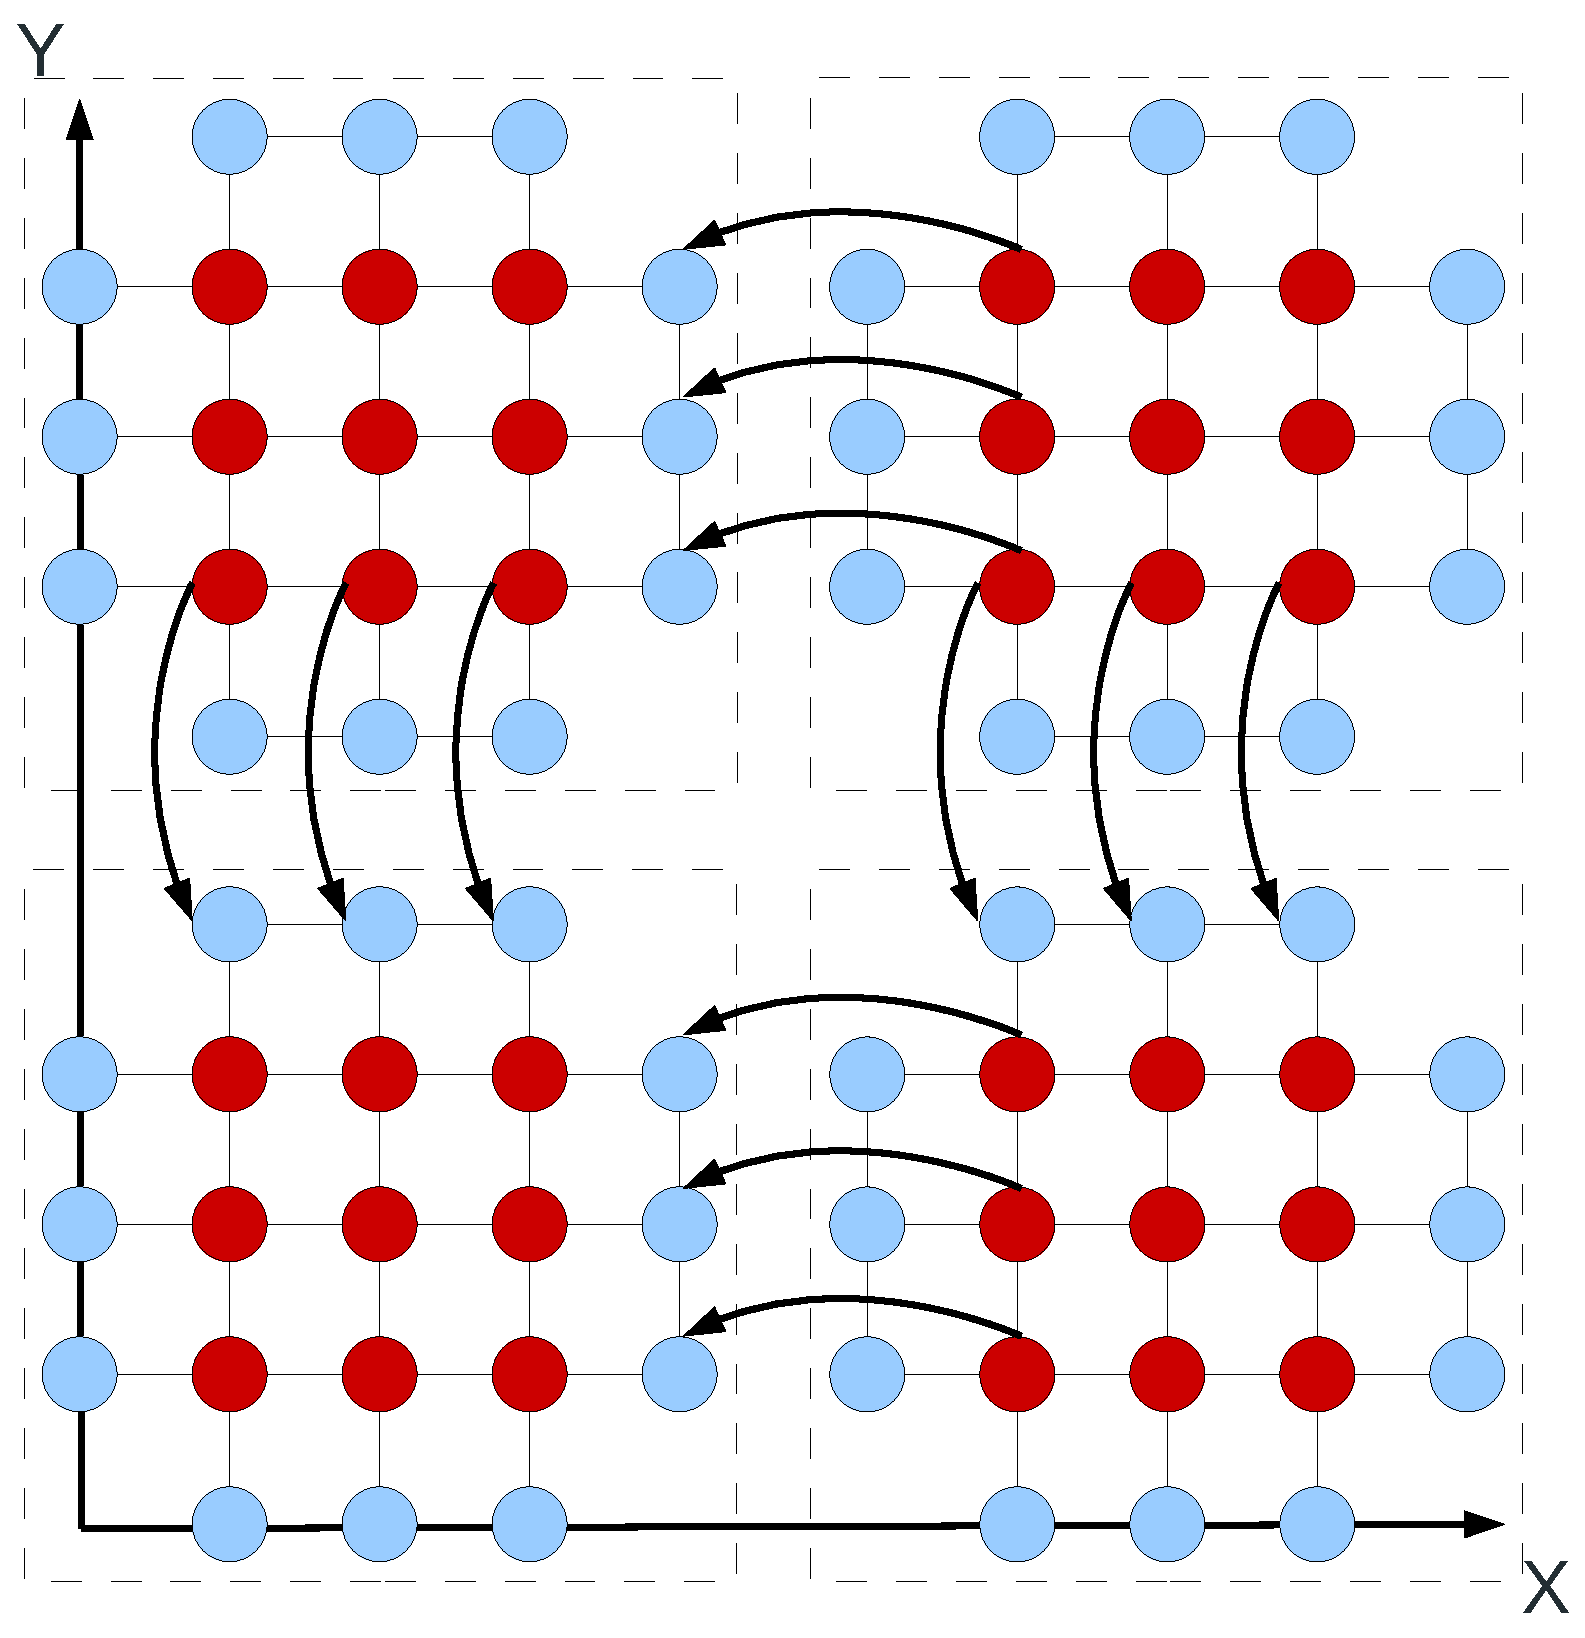
\includegraphics[height=2.5in]{artwork/pdf/decomp_4}
\end{figure}

\end{frame}